\section{Chapter 13}
%TODO: C-13.21

\begin{itemize}

      \item[R-13.1] Draw a simple undirected graph G that has 12 vertices, 18 edges, and 3
            connected components. Why would it be impossible to draw G with 3
            connected components if G had 66 edges? \\
            \answer \\
            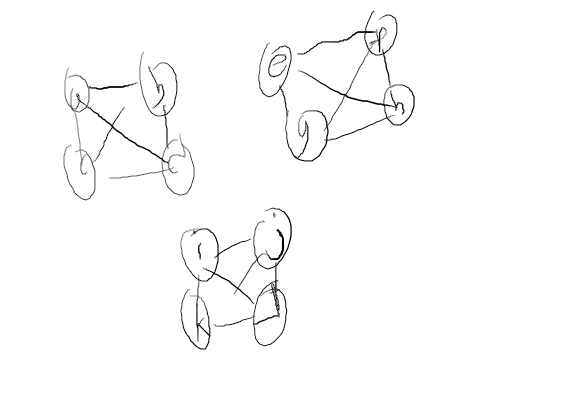
\includegraphics[scale=0.6]{img/R-13_1.png} \\
            If we consider the maximum amount of edges that G can have with 12 vertices,
            we see that it would be $\binom{12}{2} = 66$. But if there are three connected components,
            then that is equivalent to removing at least two edges from this theoretical graph and so the
            max number of edges would be 64.

      \item[R-13.3]  Draw a simple connected directed graph with 8 vertices and 16 edges such
            that the in-degree and out-degree of each vertex is 2. Show that there is
            a single (nonsimple) cycle that includes all the edges of your graph, that
            is, you can trace all the edges in their respective directions without ever
            lifting your pencil. (Such a cycle is called an Euler tour.)\\
            \answer\\
            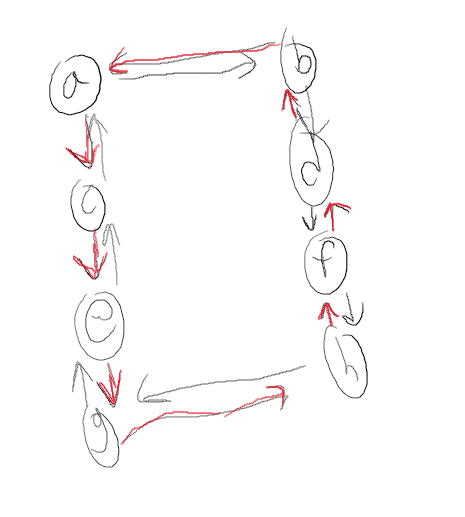
\includegraphics[scale=0.5]{img/R-13_3.png}

      \item[R-13.4]  Repeat the previous problem and then remove one edge from the graph.
            Show that now there is a single (nonsimple) path that includes all the edges
            of your graph. (Such a path is called an Euler path.)\\
            \answer\\
            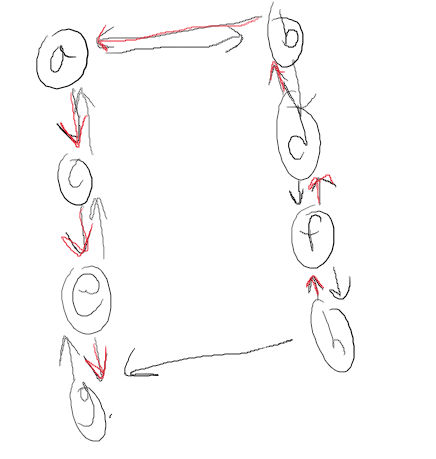
\includegraphics[scale=0.5]{img/R-13_4.png}

      \item [R-13.5]  Bob loves foreign languages and wants to plan his course schedule for the
            following years. He is interested in the following nine language courses:
            LA15, LA16, LA22, LA31, LA32, LA126, LA127, LA141, and LA169.
            The course prerequisites are:
            \begin{itemize}
                  \item LA15: (none)
                  \item LA16: LA15
                  \item LA22: (none)
                  \item LA31: LA15
                  \item LA32: LA16, LA31
                  \item LA126: LA22, LA32
                  \item LA127: LA16
                  \item LA141: LA22, LA16
                  \item LA169: LA32
            \end{itemize}
            Find the sequence of courses that allows Bob to satisfy all the prerequi-
            sites. \\
            \answer
            LA22 -> LA15 -> LA16 -> LA32 -> LA126 -> LA127 -> LA141

      \item[R-13.6]  Suppose we represent a graph G having n vertices and m edges with the
            edge list structure. Why, in this case, does the insertVertex function run
            in O(1) time while the eraseVertex function runs in O(m) time? \\
            \answer\\
            The insertVertex function runs in O(1) time because the vertices are stored in a doubly
            linked list, so insertion O(1). The eraseVertex function takes O(m) time because
            you have to check each edge and remove the ones incident to the vertex you are removing.

      \item[R-13.7] Let G be a graph whose vertices are the integers 1 through 8, and let the
            adjacent vertices of each vertex be given by the table below:
            \begin{center}
                  \begin{tabular}{c c}
                        Vertex & Adjacent Vertices \\
                        1      & (2, 3, 4)         \\
                        2      & (1, 3, 4)         \\
                        3      & (1, 2, 4)         \\
                        4      & (1, 2, 3, 6)      \\
                        5      & (6, 7, 8)         \\
                        6      & (4, 5, 7)         \\
                        7      & (5, 6, 8)         \\
                        8      & (5, 7)            \\
                  \end{tabular}

            \end{center}
            Assume that, in a traversal of G, the adjacent vertices of a given vertex are
            returned in the same order as they are listed in the table above.
            \begin{enumerate}[label=\alph*.]
                  \item Draw G.
                  \item Give the sequence of vertices of G visited using a DFS traversal starting at vertex 1.
                  \item Give the sequence of vertices visited using a BFS traversal starting at vertex 1.
            \end{enumerate}
            \answer
            \begin{enumerate}[label =\alph*.]
                  \item \text{}\\
                        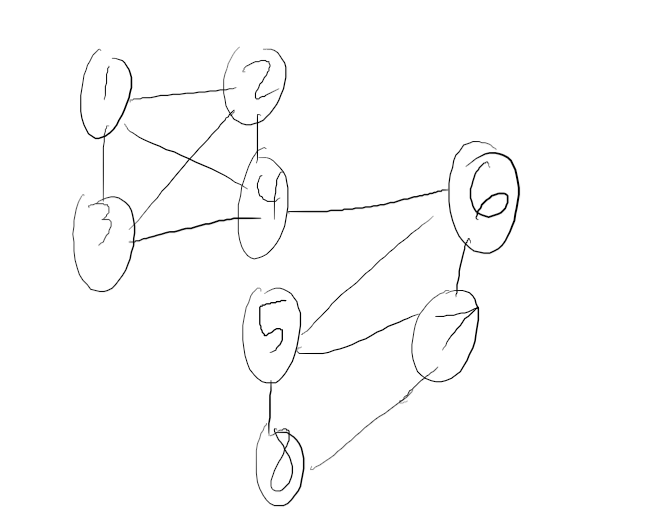
\includegraphics[scale=0.7]{img/R-13_7.png}
                  \item 1, 2, 3, 4, 6, 5, 7, 8
                  \item 1,2, 3, 4, 6, 5, 7, 8
            \end{enumerate}

      \item[R-13.8] Would you use the adjacency list structure or the adjacency matrix struc-
            ture in each of the following cases? Justify your choice.
            \begin{enumerate}[label=\alph*.]
                  \item  The graph has 10,000 vertices and 20,000 edges, and it is important
                        to use as little space as possible.
                  \item The graph has 10,000 vertices and 20,000,000 edges, and it is important to use as little space as possible.
                  \item You need to answer the query isAdjacentTo as fast as possible, no
                        matter how much space you use.
            \end{enumerate}
            \answer \\
            \begin{enumerate}[label=\alph*.]
                  \item Adjacency list because the space usage is O(n + m) where n is vertices and m is edges, while the adjacency
                        matrix has a space usage of O($n^2$) where n is vertices. So $10,000+20,000= 30,000 < 100,000,000=10,000^2$
                  \item Still adjacency list since $20,010,000 < 10,000^2$ and thus the list will take less space.
                  \item Adjacency matrix since its supports isAdjacentTo is O(1) time.
            \end{enumerate}
            \newpage
      \item[R-13.11] Compute a topological ordering for the directed graph drawn with solid
            edges in Figure 13.8(d).\\
            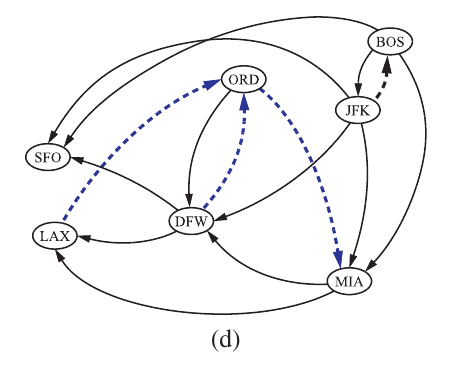
\includegraphics[scale=0.7]{img/figure_13_8_d.png} \\
            \answer\\
            BOS, JFK, MIA, ORD, DFW, SFO, LAX

      \item [R-13.29] How many edges are in the transitive closure of a graph that consists of a
            simple directed path of n vertices?\\
            \answer\\
            Vertex 1 will have n-1 edges, since it can reach every other vertex, vertex 2 will have n-2 unique edges and so on
            until vertex n-1 which has unique 1 edge and vertex n will have no new/unique edges. So the final result is
            $\sum_{i=1}^{n-1} i = \frac{(n-1)(n)}{2}$.
      \item[C-13.16] Consider the following greedy strategy for finding a shortest path from
            vertex start to vertex goal in a given connected graph.
            \begin{enumerate}
                  \item Initialize path to start.
                  \item Initialize VisitedVertices to {start}.
                  \item If start=goal, return path and exit. Otherwise, continue.
                  \item Find the edge (start,v) of minimum weight such that v is adjacent to start and v is not in VisitedVertices.
                  \item Add v to path.
                  \item Add v to VisitedVertices.
                  \item Set start equal to v and go to step 3.
            \end{enumerate}
            Does this greedy strategy always find a shortest path from start to goal?
            Either explain intuitively why it works, or give a counter example.\\
            \answer \\
            No, this greedy algorithm does not work. For example with this graph: \\
            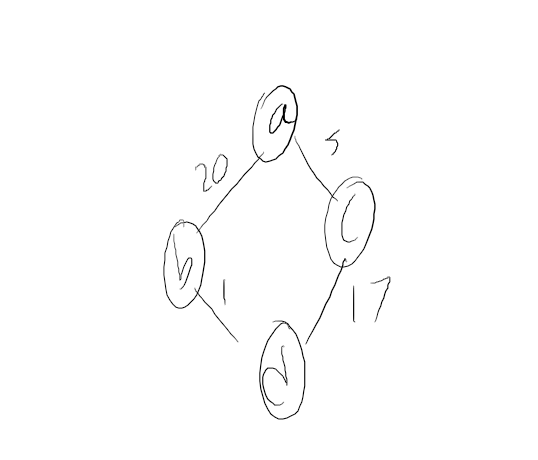
\includegraphics[scale =.7]{img/C-13_16.png} \\
            If we start at vetex a and want to reach d, it will go to c since $5<20$
            and then go to d. However, that path has a total weight of 22 and if it went to b then d,
            it would have a better total weight of 21.

      \item[C-13.21] NASA wants to link n stations spread over the country using communication
            channels. Each pair of stations has a different bandwidth available,
            which is known a priori. NASA wants to select n - 1 channels (the minimum
            possible) in such a way that all the stations are linked by the channels
            and the total bandwidth (defined as the sum of the individual bandwidths
            of the channels) is maximum. Give an efficient algorithm for this problem
            and determine its worst-case time complexity. Consider the weighted
            graph G = (V, E), where V is the set of stations and E is the set of chanels
            between the stations. Define the weight w(e) of an edge e in E as the
            bandwidth of the corresponding channel.\\
            \answer\\
            You can use a variation of the PrimJarnik minimum spanning tree algorithm.
            Insead of setting the iniital distance/key to infinity you can set it to negative infinity
            even negative 1 assuming no negative bandwidth. Then for the edge relaxtion you will update
            the value when the weight is greater than the key. This will have the same running time of $O(m\log n)$.



\end{itemize}